\documentclass[11pt, oneside]{article}   	% use "amsart" instead of "article" for AMSLaTeX format
\usepackage{geometry}                		% See geometry.pdf to learn the layout options. There are lots.
\geometry{letterpaper}                   		% ... or a4paper or a5paper or ... 
%\geometry{landscape}                		% Activate for for rotated page geometry
%\usepackage[parfill]{parskip}    		% Activate to begin paragraphs with an empty line rather than an indent
\usepackage{graphicx}				% Use pdf, png, jpg, or eps� with pdflatex; use eps in DVI mode
								% TeX will automatically convert eps --> pdf in pdflatex		
\usepackage{amssymb}
\usepackage{amsmath}

\title{Arcs of a circle}
%\author{The Author}
\date{}							% Activate to display a given date or no date

\graphicspath{{/Users/telliott_admin/Dropbox/Tex/png/}}

\begin{document}

\maketitle
%\section{}
% \subsection*{R code}
% \begin{lstlisting}  \end{lstlisting}
% \begin{center} 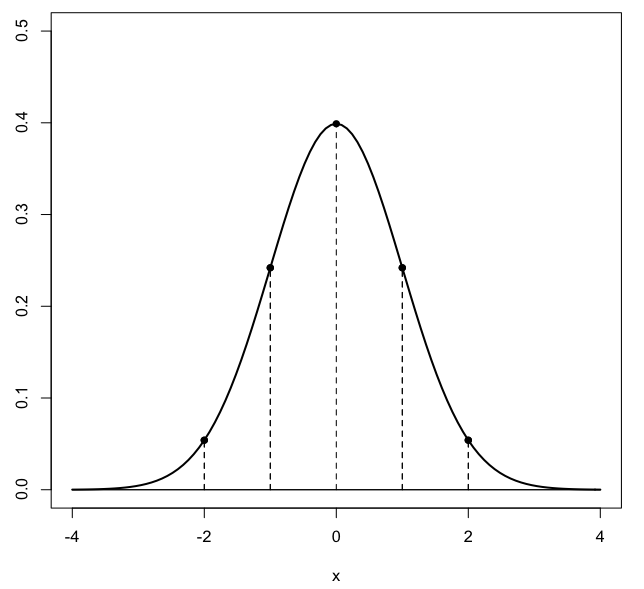
\includegraphics [scale=0.4] {gauss3.png} \end{center}
% \begin{bmatrix} a  &  b \\ c  &  d \end{bmatrix}
% \bigg |_

\large
\noindent
\begin{center} 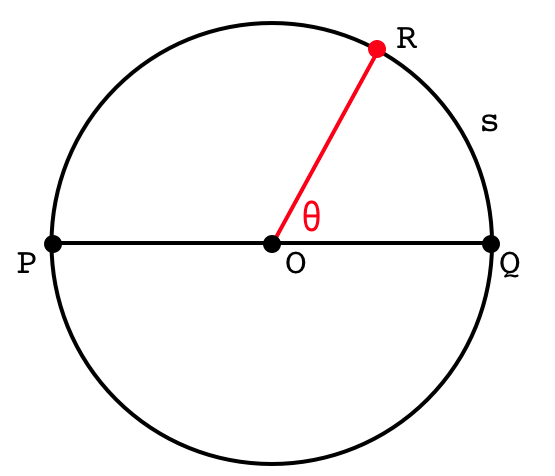
\includegraphics [scale=0.4] {arcs1.png} \end{center}
In calculus and analytical geometry angles are defined in terms of radians of arc. For a unit circle with radius = $1$, the total circumference is $2\pi$, so the arc swept out by the angle $\theta$ is in the same ratio to $\pi$ as the ratio of the angle's measure in degrees to $180^\circ$. We say that the angle $\theta$ in this figure is equal to the arc it sweeps out on the circumference.
\[ s = \theta \]
We substitute measures of angles in radians for the ones in degrees:

\[ 180^\circ = \pi, \ 90^\circ = \frac{\pi}{2} \]
\[ 60^\circ = \frac{\pi}{3}, \ 45^\circ = \frac{\pi}{4}, \ 30^\circ = \frac{\pi}{6} \]
Now, think of the same points on the circumference of the circle as forming a triangle. If two points are on a diameter of the circle, the angle at any third point is always a right angle.

To prove: $\angle PRQ$ is a right angle.
\begin{center}
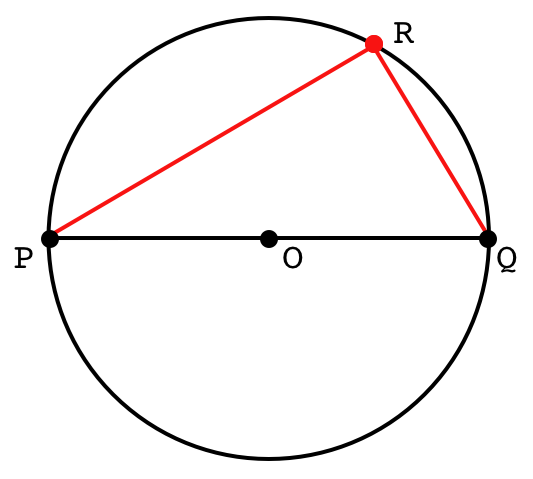
\includegraphics [scale=0.4] {arcs2.png} 
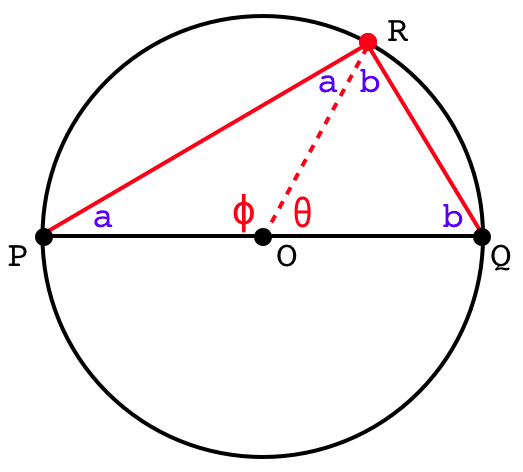
\includegraphics [scale=0.4] {arcs3.png}
\end{center}
Solution:
Draw the radius OR. Notice that $\triangle OPR$ and $\triangle OQR$ are both isosceles.
Label the respective base angles $a$ and $b$. By considering that they comprise the angles of $\triangle PQR$:
\[ 2a + 2b  = \pi \]
\[ a + b = \frac{\pi}{2} \]

In addition, the arcs swept out by angles $a$ and $b$ (OPR and OQR on the diameter) clearly add up to $\pi$. This suggests that:

\[ a = \frac{\theta}{2} \]
\[ b = \frac{\phi}{2} \]

Solution:

\[ 2a + 2b = \pi = 2a + \phi \]
\[ \phi = 2b \]
Consider the chord PR and draw the tangent at P.
\begin{center} 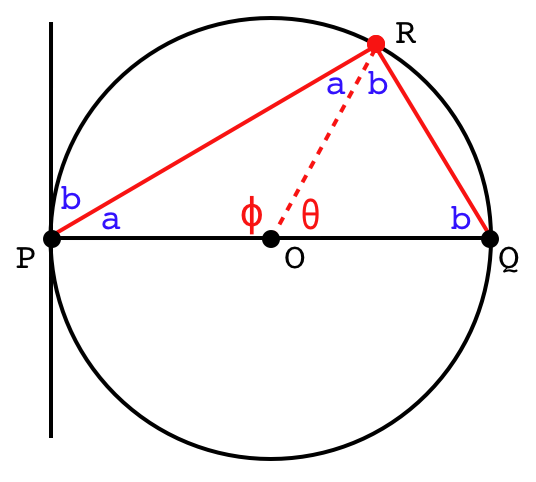
\includegraphics [scale=0.4] {arcs4.png} \end{center}
The arc between the tangent and the chord equals 2b because it is the same arc as cut off by $\angle \ PQR$ (which is $\angle \ b$).

Take a chord of the circle, draw the diameter and the tangent.
The same rule applies to both angles: one between the chord and the diameter, and the second between the chord and the tangent. The arc is twice the measure of the angle.

\subsection*{Generalized arc}

Having established these basic facts we can do a bit more.
One is to generalize the result for all arcs. The examples so far contain the diameter in some way. Consider the arc swept out by the angle $\theta$ in this figure.
\begin{center} 
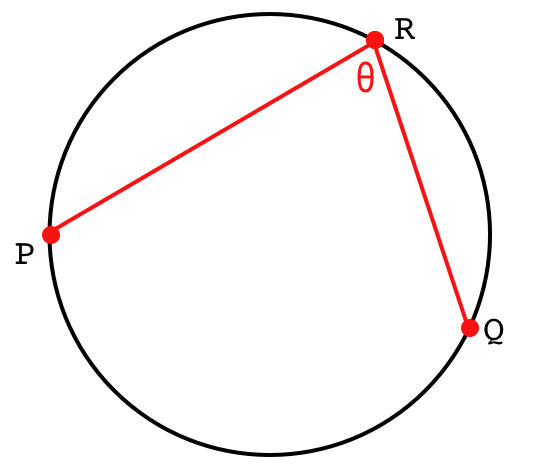
\includegraphics [scale=0.35] {arcs5.png} 
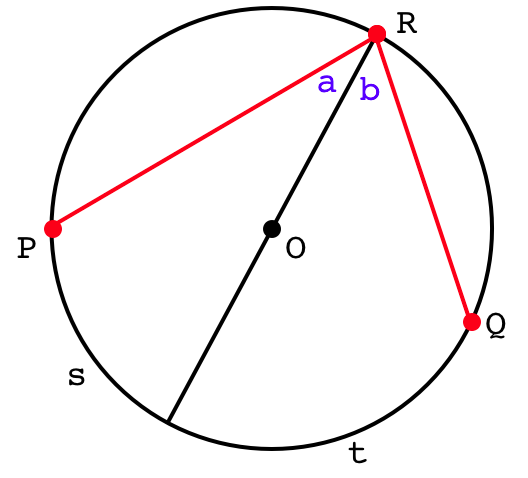
\includegraphics [scale=0.35] {arcs6.png}
\end{center}
We can prove that the measure of the angle $\theta$ is equal to the 1/2 the arc swept out between P and Q. For a simple proof, draw the diameter:
By our previous work:

\[ b = \frac{t}{2} \]
\[ a = \frac{s}{2} \]
\[ \theta = a + b = \frac{s+t}{2} \]

\subsection*{Intersecting chords}
Given two chords,
to prove:

\[ \theta = 1/2 (s + t) \]

\begin{center} 
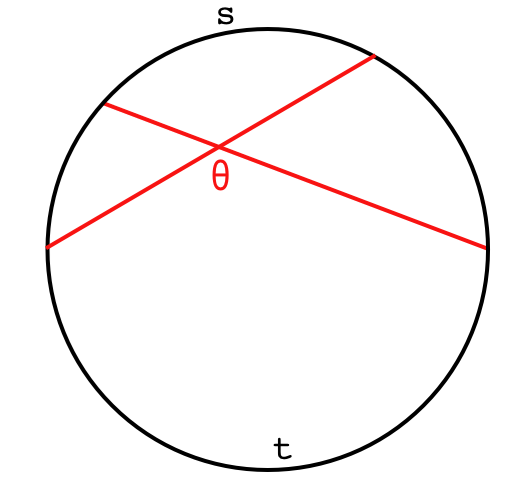
\includegraphics [scale=0.4] {arcs7.png} 
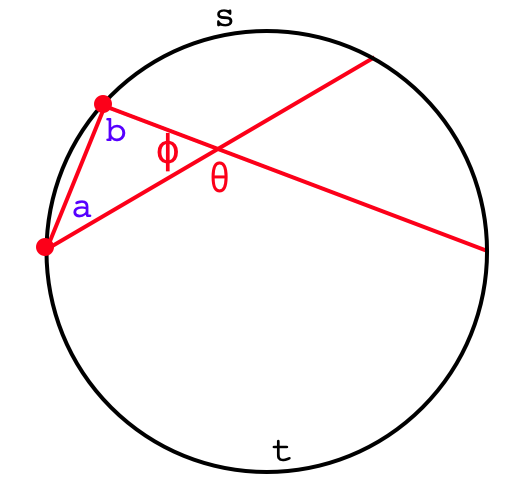
\includegraphics [scale=0.4] {arcs8.png}
\end{center}

$\theta$ is the average of the two arc lengths.
Solution:
Draw a triangle.

\[ a = \frac{s}{2} \]
\[ b = \frac{t}{2} \]
\[ a + b = \theta = \frac{s+t}{2} \]

\subsection*{Tangent and secant}

Rather than having all three points on the circle, one is now outside. We have the same arc swept out by the endpoints ($t$), but the included angle is now smaller, and there is a new small piece of arc length $s$.

\begin{center} 
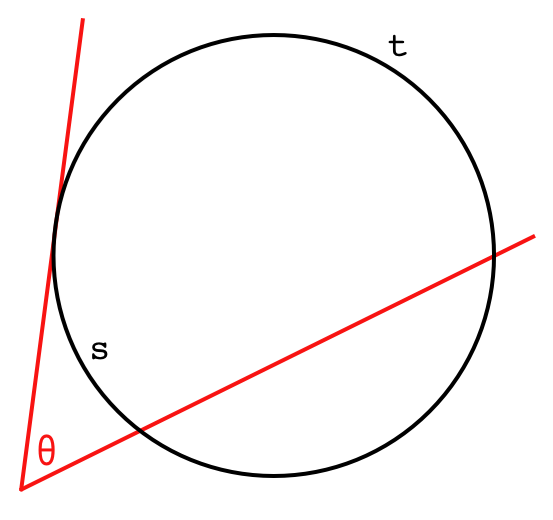
\includegraphics [scale=0.35] {arcs9.png} 
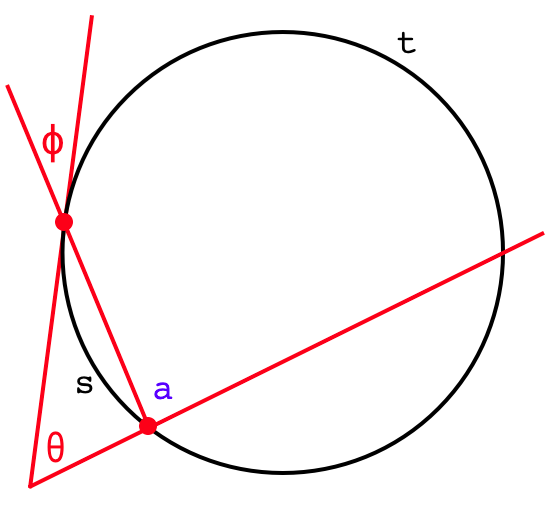
\includegraphics [scale=0.35] {arcs10.png}
\end{center}

To prove:

\[ \theta = \frac{t-s}{2} \]

Solution:
Draw the triangle.
By our previous work (and supplementary angles):

\[ \phi = \frac{s}{2} \]
\[ a = \frac{t}{2} \]

by supplementary angles:

\[ \theta + \phi = a \]
\[ \theta = \frac{t}{2} - \frac{s}{2} \]
\[ = \frac{t-s}{2} \]
\subsection*{Two tangents}
\begin{center} 
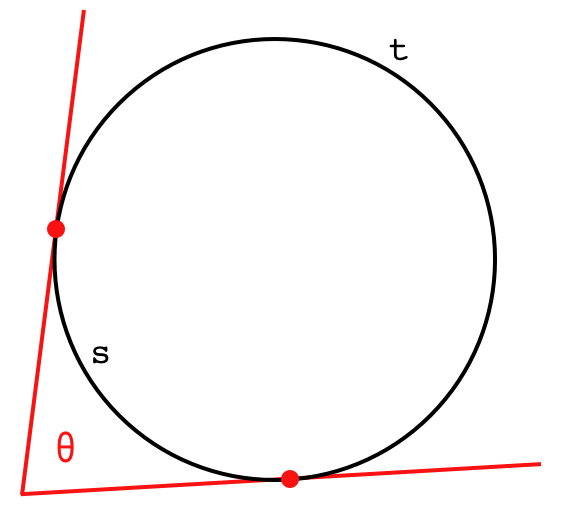
\includegraphics [scale=0.35] {arcs11.png} 
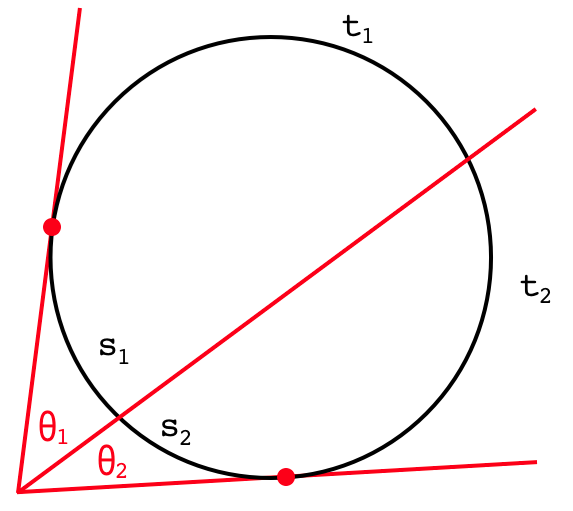
\includegraphics [scale=0.35] {arcs12.png}
\end{center}
Draw a secant line
By our previous work:

\[ \theta_1 = \frac{t_1 - s_1}{2} \]
\[ \theta_2 = \frac{t_2 - s_2}{2} \]

By addition:

\[ \theta = \frac{t - s}{2} \]
\subsection*{Two secants}

\begin{center} 
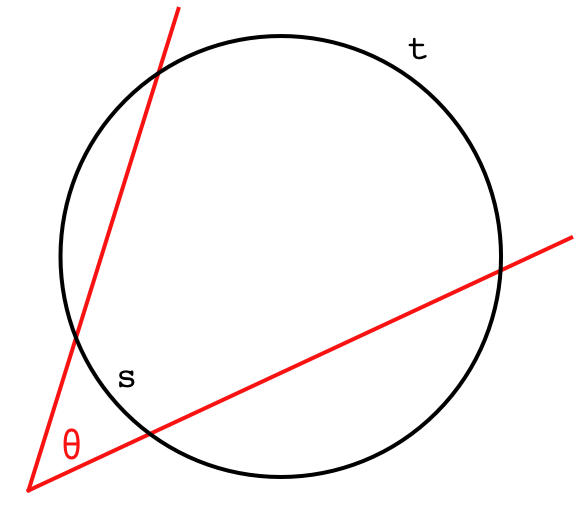
\includegraphics [scale=0.35] {arcs13.png} 
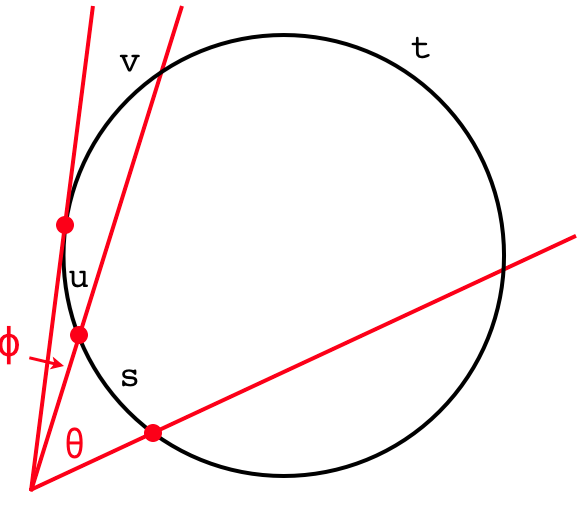
\includegraphics [scale=0.35] {arcs14.png}
\end{center}
Draw a tangent line.
By our previous work:

\[ \theta + \phi = \frac{t - s}{2} + \frac{v - u}{2} \]
\[ \phi = \frac{v - u}{2} \]

By subtraction:

\[ \theta = \frac{t - s}{2} \]

\subsection*{Chord segments}

Finally, there is a simple algebraic relationship between chord segments. Draw two chords of the circle and label the lengths of the segments as shown (note: $s$ and $t$ do not refer to arcs any more).

\begin{center} 
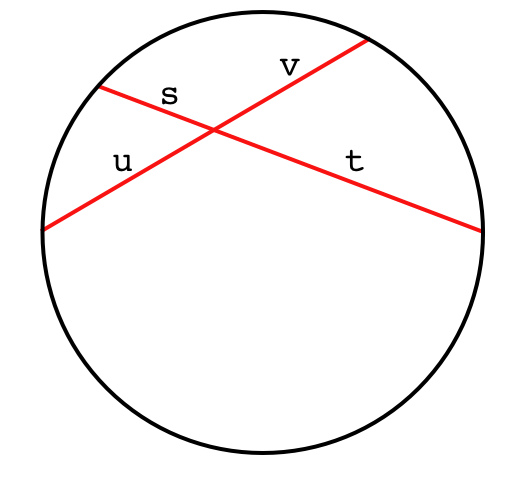
\includegraphics [scale=0.35] {arcs15.png} 
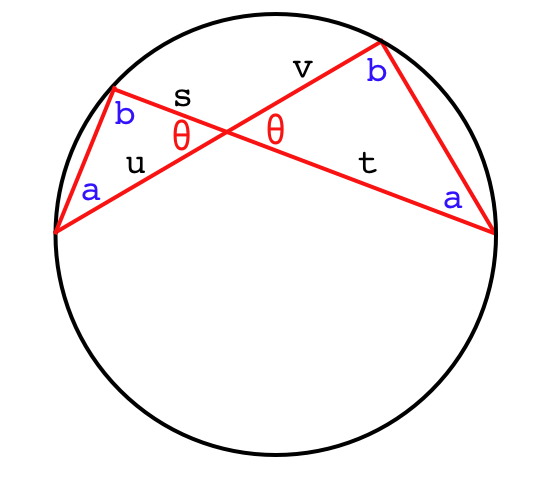
\includegraphics [scale=0.35] {arcs16.png}
\end{center}
To prove:

\[ st = uv \]

Solution:
Draw the two triangles.
Notice that the two angles labeled $a$ are equal because they sweep out the same arc of the circle, and similarly for the two angles labeled $b$. By similar triangles:

\[ s/u = v/t \]
\[ st = uv \]

\end{document}  